\documentclass{recipe}

\begin{document}
\begin{recipe}{Swedish Meatballs}
  \servings{32}

  \begin{ingredients}
    \ingredient{}{}{breadcrumbs}
    \ingredient{2}{large}{eggs}
    \ingredient{}{}{milk}
    \ingredient{}{}{nutmeg}
    \ingredient{}{}{allspice}
    \ingredient{}{}{salt}
    \ingredient{1}{lb}{ground beef}
    \ingredient{1}{lb}{ground pork}
    \ingredient{}{}{butter}
    \ingredient{}{}{flour}
    \ingredient{}{}{beef stock}
    \ingredient{}{}{milk}
  \end{ingredients}

  \begin{images}
    \begin{image}
      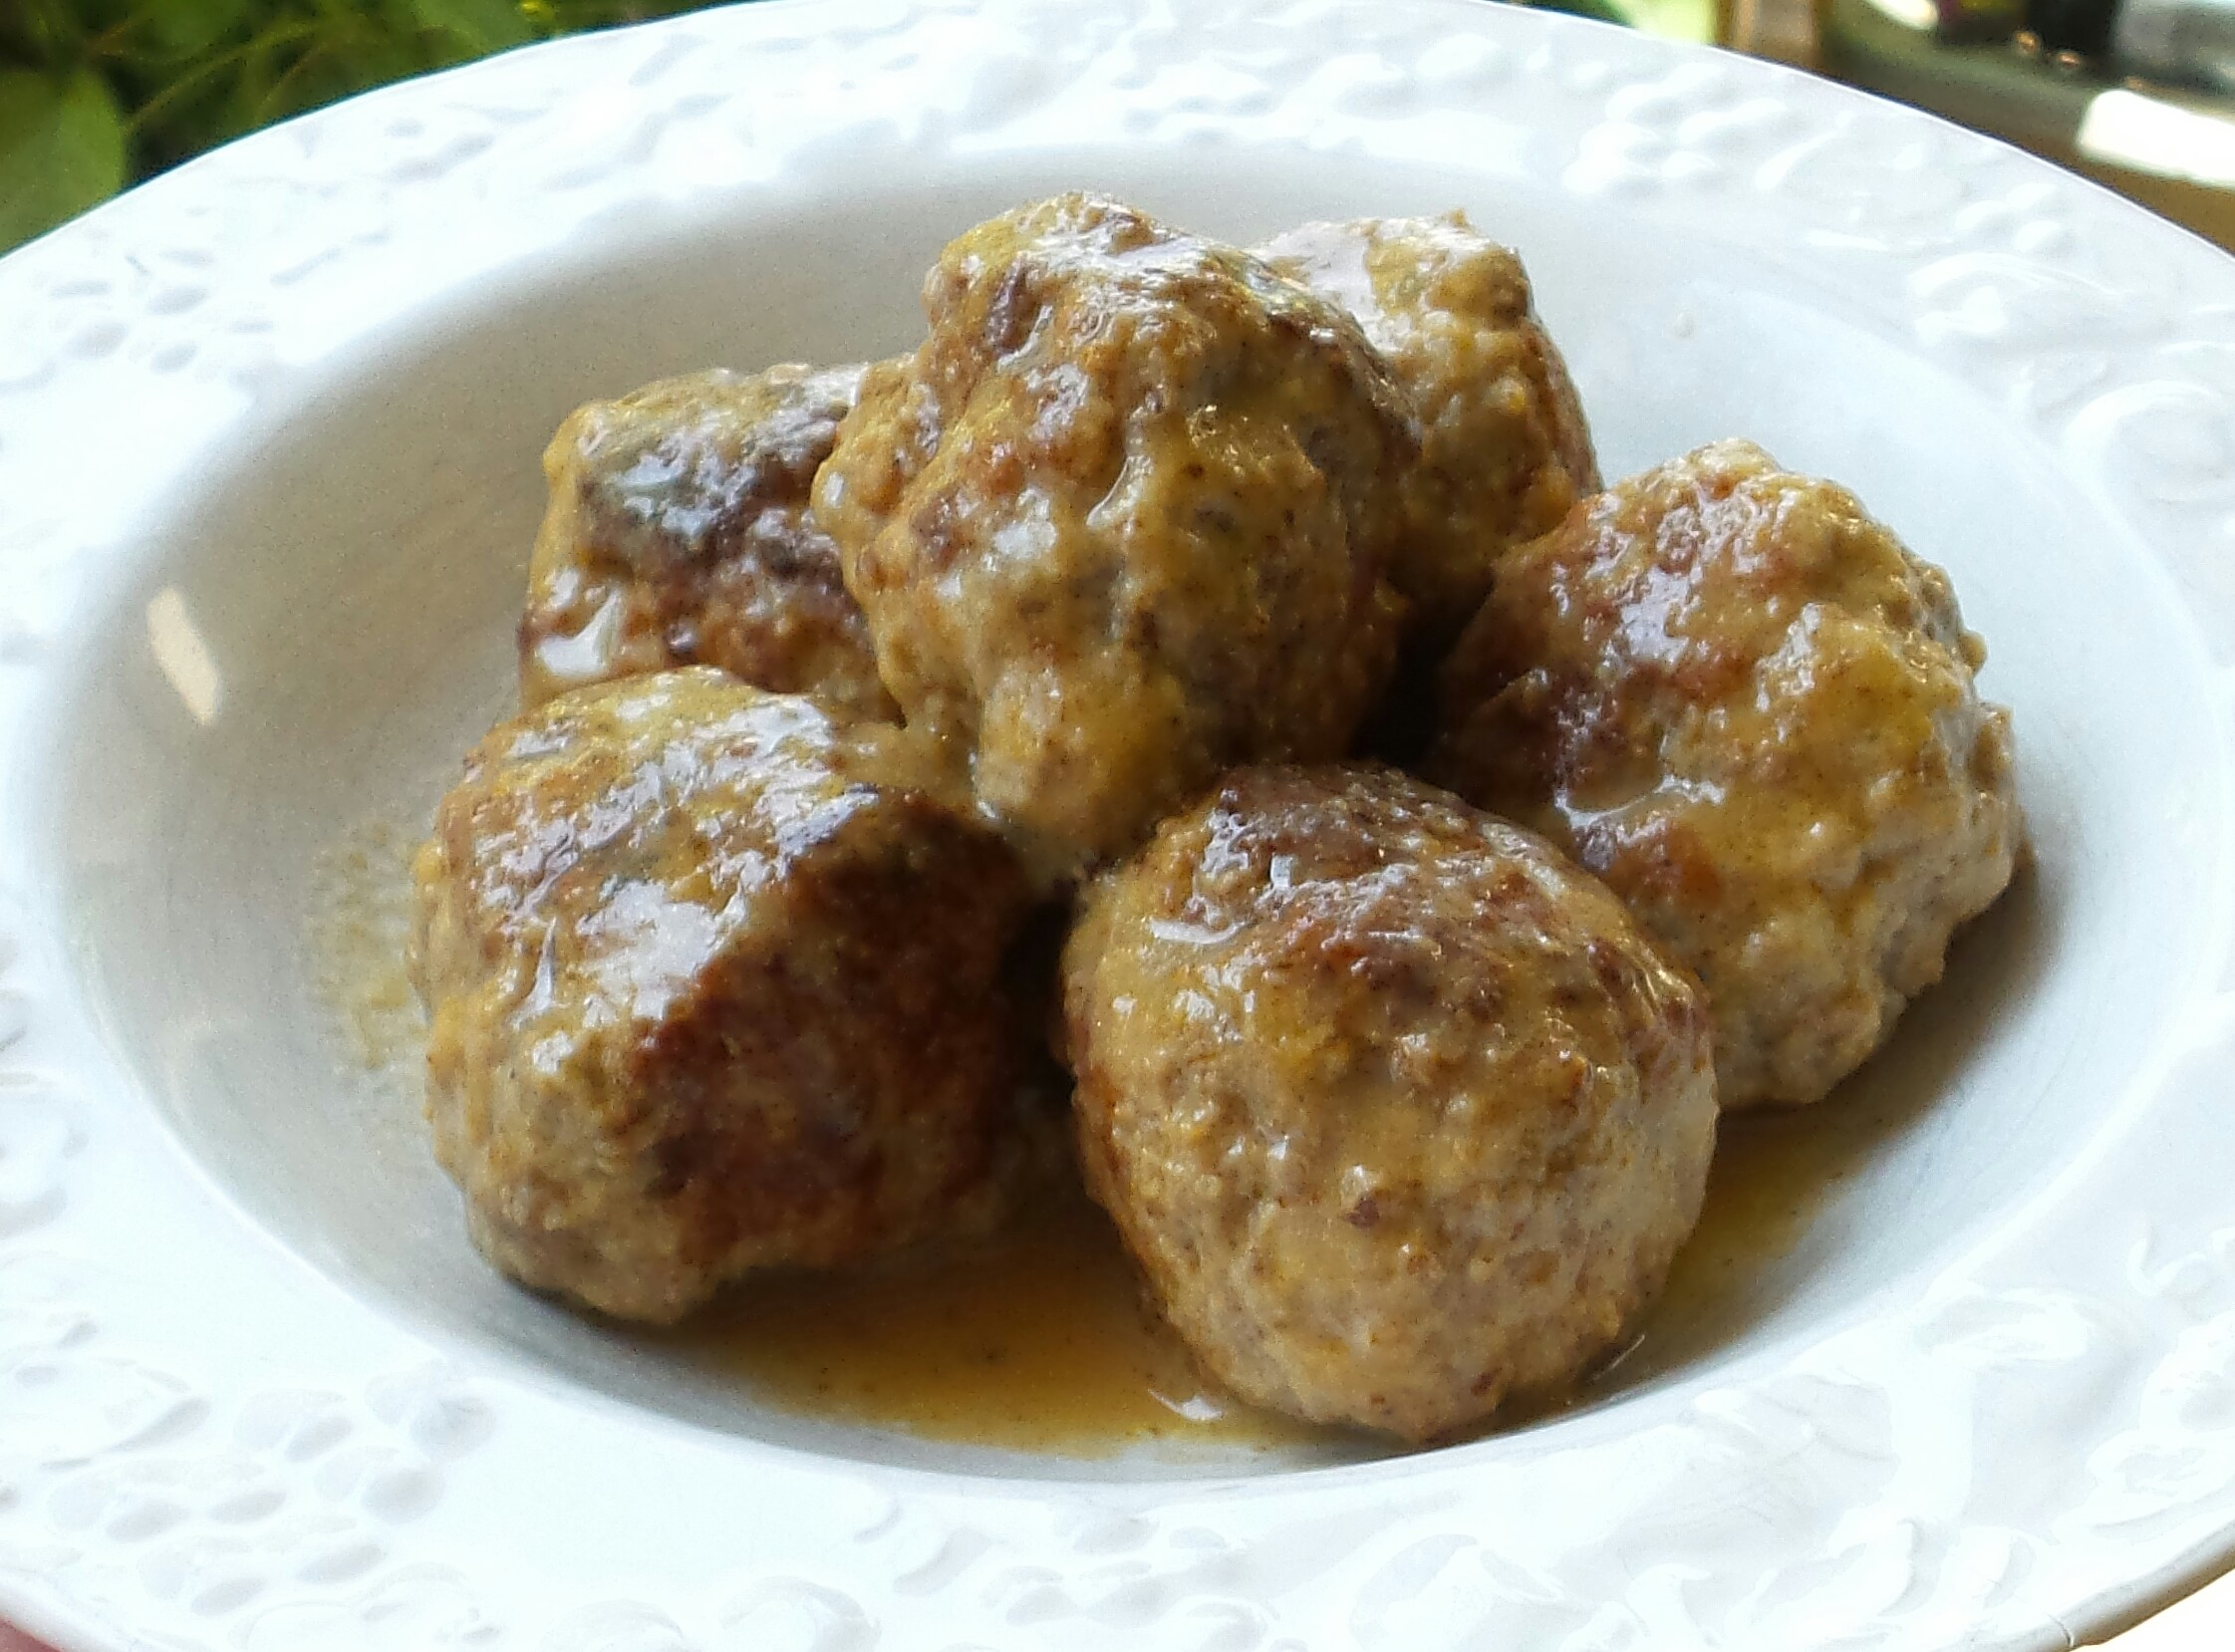
\includegraphics[width=\linewidth,trim=0px 0px 0px 0px, clip=true]{swedish_meatballs-01.jpeg}
    \end{image}
  \end{images}

  \begin{steps}
  \item Mix the breadcrumbs, eggs, milk, nutmeg, allspice and salt
    together until a slurry is formed.
  \item Incorporate the meat into the slurry.
  \item Put the meat mixture into the fridge for an hour to cool down.
  \item Form meatballs from the meat mixture.
  \item Brown the meatballs in butter, then remove them from the pan.
  \item Make a roux from the flour and the remaining fat.
  \item Thin the roux with the beef stock to form a gravy.
  \item Return the meatballs to the pan and simmer for 15 minutes,
    skimming as much fat as possible.
  \item Add milk to the gravy until it reaches the desired color.
  \end{steps}

  \begin{notes}
  \item I put cloves instead of allspice, and I don't think this was good.
  \item There was too much fat in the sauce, more flour and maybe some
    onions would have helped.
  \item I should have mixed the meat a bit less, the meatballs were a
    bit tough.
  \end{notes}
\end{recipe}
\end{document}
